\documentclass{beamer}

\usepackage{txfonts}
\usepackage{hyperref}
\usepackage{fancybox}
\usepackage{xfrac}
\usepackage{cancel,slashbox}

\newcommand{\heart}{\ensuremath\heartsuit}

\usepackage{mathtools,amssymb}
\newcommand{\myarrow}{\scalebox{2}[2]{$\mathclap{\curvearrowleft}\mkern2.2mu
                                                 \mathclap{\curvearrowright}$}}

\DeclareMathOperator{\Bin}{\mathrm{Bin}}
\DeclareMathOperator{\Max}{\mathrm{Max}}
\DeclareMathOperator{\Cov}{\mathrm{Cov}}
\DeclareMathOperator{\Covr}{\mathrm{Covr}}
\DeclareMathOperator{\Corr}{\mathrm{Corr}}

\hypersetup{colorlinks=false,linkbordercolor=red,linkcolor=green,pdfborderstyle={/S/U/W 1}}

\addtobeamertemplate{navigation symbols}{}{ \hspace{1em}    \usebeamerfont{footline}%
    \insertframenumber / \inserttotalframenumber}

\geometry{papersize={15cm,15cm}}
\usepackage{lipsum}

\makeatletter
\newenvironment<>{contdproof}[1][\proofname]{%
    \par
    \def\insertproofname{#1\@addpunct{.}}%
    \usebeamertemplate{proof begin}#2}
  {\usebeamertemplate{proof end}}
\makeatother


\setbeamertemplate{theorems}[numbered]

\newtheorem{remark}{Remark}



\newtheorem*{nonumdefinition}{Definition}
\newtheorem*{nonumproblem}{Problem}
\newtheorem*{nonumcorollary}{Corollary}
\newtheorem*{nonumlemma}{Lemma}
\newtheorem*{nonumproof}{Proof}
\newtheorem*{nonumtheorem}{Theorem}
\newtheorem*{nonumremark}{Remark}
\newtheorem*{answer}{Answer}
\newtheorem*{nonumremarks}{Remarks}
\newtheorem*{nonumexamples}{Examples}
\newtheorem*{nonumsolution}{Solution}
\newtheorem*{nonumexample}{Example}
\newtheorem*{nonumproposition}{Proposition}
\newtheorem{proposition}[theorem]{Proposition}

\usepackage{tikz}
\newcommand*\mycirc[1]{%
  \tikz[baseline=(C.base)]\node[draw,circle,inner sep=.7pt](C) {#1};\:
}

\newcommand\myheading[1]{%
  \par\bigskip
  {\color{blue}{\large #1}}\par\smallskip}

%\usetheme{Warsaw}
%\usetheme{Berkeley} %sample 1

\usetheme{Berlin} % sample 2
%\usetheme{AnnArbor} % sample 3

\let\otp\titlepage
\renewcommand{\titlepage}{\otp\addtocounter{framenumber}{-1}}

\title{Lecture 17 : Double Integrals}
\author{}
\date{}

\begin{document}
\begin{frame}[plain]
\titlepage
\end{frame}

\begin{frame}
Some of you have not learned how to do double integrals. In this course you will need to do double integrals over rectangles and I will now explain how to do such calculations.

\myheading{Partial (Indefinite) Integration}

In one variable calculus you learned about the indefinite integral $\int f(x)dx$. The point of the indefinite integral was that it was an inverse of the derivative
$$
\frac{d}{dx}\left(\int f(x)dx\right)=f(x)
$$
(In fact this is the definition of the) indefinite integral.
\end{frame}

\begin{frame}
So
$$
\int x^{3}dx=\dfrac{x^{4}}{4}
$$
and
$$
\dfrac{d}{dx}\dfrac{x^{4}}{4}=x^{3}
$$
The indefinite integral is defined only up to an arbitrary constant, ``the constant of integration''.

The fundamental theorem of calculus then says that to evaluate the \underline{definite} integral $\int\limits^{b}_{0}f(x)dx$ you take \underline{any indefinite} integral, evaluate it at the upper limit $b$ and at the lower limit $a$ and subtract the latter from the former.
\end{frame}

\begin{frame}
Now in two variable calculus you have \underline{two} ``partial'' derivatives $\dfrac{\partial f}{\partial x}(x,y)$ and $\dfrac{\partial f}{\partial y}(x,y)$ so you have two partial indefinite integrals $\int f(x,y)dx$ and $\int f(x,y)dy$. 

So (by definition)
\begin{align*}
\frac{\partial}{\partial x}\left(\int f(x,y)dx\right)=f(x,y)\\
\frac{\partial}{\partial y}\left(\int f(x,y)dy\right)=f(x,y).
\end{align*}
Let's compute 
$$
\int (x^{2}+y^{2})dx.
$$
The idea is to \underline{tract $y$ as a constant.}
\end{frame}

\begin{frame}

\centerline{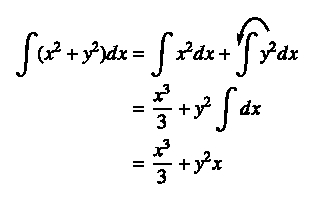
\includegraphics{figure/fig1.eps}}
\smallskip

The partial indefinite integral in $x$ is \underline{defined only up to a function of $y$.} (because $\dfrac{\partial}{\partial x}g(y)=0$).

Let's do a harder one 
$$
\int \sin xy \ dy=-\dfrac{1}{x}\cos xy.
$$

\smallskip
\centerline{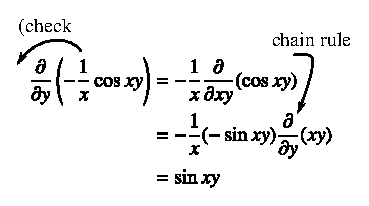
\includegraphics{figure/fig2.eps}}
\end{frame}

\begin{frame}
\myheading{Partial (Definite) Integrals}

Once you have the partial indefinite integral you have the partial definite integral
\begin{align*}
\int\limits^{2}_{1}(x^{2}+y^{2})dx &= \left(\frac{x^{3}}{3}+y^{3}x\right)\Big|^{x=2}_{x=1}\\[3pt]
                                &= \left(\frac{8}{3}+2y^{2}\right)-\left(\frac{1}{3}+y^{2}\right)\\[3pt]
                                &= y^{2}+\frac{7}{3}
\end{align*}

\myheading{The Golden Rule}

Treat $y$ as a constant throughout and do the one variable integral with respect to $x$.

Note \underline{the output is a function of $y$.}
\end{frame}

\begin{frame}
\myheading{Using Partial Integration to Evaluate Double Integrals over Rectangles}

Just as we use the indefinite integral in one variable to evaluate definite integrals in one variable we will use the partial integrals to evaluate (definite) double integrals
\begin{equation*}
\begin{tabular}{c}
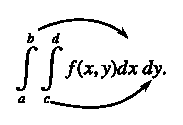
\includegraphics{figure/fig3.eps}
\end{tabular}\tag{*}\label{eq=*}
\end{equation*}

The notation is very confusing because of tradition. Here the $x$-limits are $a$ and $b$ and the $y$-limits are $c$ and $d$ \underline{so $a$ and $b$ go with $dx$ and $c$ and $d$ go with $dy$.}

\underline{Watch out for this later.}
\end{frame}

\begin{frame}
So we have a rectangle $R$ $[a,b]\times [c,d]$ in the $xy$-plane

\smallskip
\centerline{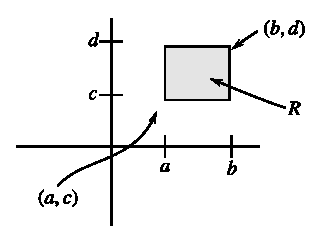
\includegraphics{figure/fig4.eps}}
\smallskip

When you learn integration theory correctly you will write this integral as
\begin{equation*}
\int\int\limits_{R} f(x,y) dx \ dy\tag{**}\label{eq-**}
\end{equation*}
However putting in the limits $a$, $b$ and $c$, $d$ is helpful for computations. Think of rewriting \eqref{eq-**} as
$$
\int\limits^{x=b}_{x=a}\int\limits^{y=d}_{y=c}f(x,y)dx \ dy.
$$
\end{frame}

\begin{frame}
So how do you compute
\begin{equation*}
\int\limits^{2}_{1}\int\limits^{1}_{0}(x^{2}+y^{2})dx \ dy\tag{**}\label{addeq-**}
\end{equation*}
So the rectangle $R$ is a square 

\smallskip
\centerline{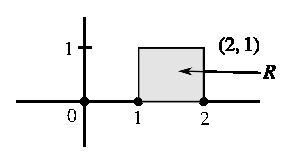
\includegraphics{figure/fig5.eps}}
\smallskip

Here is how you compute \eqref{addeq-**}.

There are \underline{two} ways. It is a famous theorem of Fubini that they lead to the same result. We will see this in our example. \underline{Pick the way that leads to the easiest computations.}
\end{frame}

\begin{frame}
\myheading{First way (do the $x$-integration first)}

\begin{enumerate}
\item Write \eqref{addeq-**} as

\smallskip
\centerline{\includegraphics{figure/fig6.eps}}
\smallskip

{\Large Z} Remember $1$ and $2$ go with $dx$ and $0$ and $1$ go with $dy$ (see page 6)

\item Do the inside partial definite integral. The output will be the function of $y$ $g(y)=y^{2}+\dfrac{7}{3}$ (from page 5).
\end{enumerate}
\end{frame}

\begin{frame}
\begin{enumerate}
\setcounter{enumi}{2}
\item Do a one variable definite integral of $g(y)$ with respect to $y$ from $0$ to $1$.
\begin{align*}
\int\limits^{1}_{0}\left(y^{2}+\frac{7}{3}\right)dy &= \left.\left(\frac{y^{3}}{3}+\frac{7}{3}y\right)\right|^{y=0}_{y=0}\\[3pt]
&= \frac{1}{3}+\frac{7}{3}=\frac{8}{3}
\end{align*}
That's it.
\end{enumerate}
The above method is said to evaluate the double integral by iterated one variable integrals.

\underline{However the first step is new it is a partial integral with respect to $x$.}
\end{frame}

\begin{frame}
\myheading{Second way (do the $y$-integration first)}

\begin{enumerate}
\item This time we write \eqref{addeq-**} as

\smallskip
\centerline{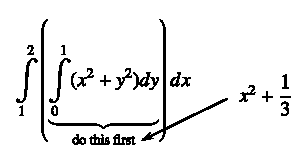
\includegraphics{figure/fig7.eps}}
\smallskip

\item Now we do the partial integration with respect to $y$ so \underline{$x$ is a constant.}
\begin{align*}
\int\limits^{1}_{0}(x^{2}+y^{2})dy &= \left.\left(x^{2}y+\frac{y^{3}}{3}\right)\right|^{y=1}_{y=0}\\[3pt]
                                &= x^{2}+\frac{1}{3}
\end{align*}
The output is a function of $x$.
\end{enumerate}
\end{frame}

\begin{frame}
\begin{enumerate}
\setcounter{enumi}{2}
\item Perform the one variable integration of the output function $h(x)=x^{2}+\frac{1}{3}$ with respect to $x$.
\begin{align*}
\int\limits^{2}_{1}\left(x^{2}+\frac{1}{3}\right)dx &= \left.\left(\frac{x^{3}}{3}+\frac{x}{3}\right)\right|^{x=2}_{x=1}\\[3pt]
 &= \left(\frac{8}{3}+\frac{2}{3}\right)-\left(\frac{1}{3}+\frac{1}{3}\right)\\[3pt]
 &= \frac{8}{3}
\end{align*}
So as predicted we got the same answer no matter which order we chose to perform the iterated integrals.
\end{enumerate}
\end{frame}

\begin{frame}
\myheading{Double Integrals of Product Functions over Rectangles}

There is one case in which double integrals one particularly easy to compute.

\begin{nonumdefinition}
Let $f(x,y)$ be a function of two variables $x$ and $y$. The $f(x,y)$ is a product function if there exist $g(x)$ and $h(g)$ such that
$$
f(x,y)=g(x)h(y)
$$
\end{nonumdefinition}
\end{frame}

\begin{frame}
\begin{nonumexamples}
\begin{alignat*}{2}
& f(x,y) = e^{x}\sin y &\qquad& \text{YES (it is a product)}\\[3pt]
& f(x,y) = e^{x}+\sin y &\qquad& \text{NO (it is not a product)}\\[3pt]
& f(x,y) = xy           &\qquad& \text{YES}\\[3pt]
& f(x,y) = x+y          &\qquad& \text{NO}
\end{alignat*}
\end{nonumexamples}

\begin{nonumtheorem}
\begin{align*}
& \int\limits^{b}_{a}\int\limits^{d}_{c}(g(x)h(y))dx \ dy\\[3pt]
&\qquad \left(\int\limits^{b}_{a}g(x)dx\right)\left(\int\limits^{d}_{c}h(y)dy\right)
\end{align*}
{\Large Z} Most functions of $x$ and $y$ are NOT product functions.
\end{nonumtheorem}
\end{frame}

\begin{frame}
\begin{nonumtheorem}[Cont.]
So
\begin{align*}
\int\limits^{1}_{0}\int\limits^{1}_{0}(xy^{2})dx \ dy &= \left(\int\limits^{1}_{0}x \ dx\right)\left(\int\limits^{1}_{0}g^{2}dy\right)\\[3pt]
&= \left(\frac{1}{2}\right)\left(\frac{1}{3}\right)=\frac{1}{6}
\end{align*}
So a double integral of a product function over a rectangle is the product of two one variable integrals (one in $x$, the other in $y$).
\end{nonumtheorem}
\end{frame}
\end{document}


